
\documentclass[11pt, a4paper]{article}
%\usepackage{proj1}
\usepackage{natbib}
\usepackage{fancyhdr}  
\usepackage{subcaption}
\usepackage{caption}
\usepackage{graphicx}
\usepackage{numprint}
\usepackage{multirow}
\linespread{1.25} 
\setlength{\parindent}{0cm}
\graphicspath{{Images/}}
\usepackage{hyperref}
\usepackage{amsmath}
\usepackage{amsfonts}
\usepackage{amssymb}
\usepackage{amsthm}
\usepackage{mathtools}
\usepackage{commath}
\usepackage{bbm}

%\usepackage[sc,osf]{mathpazo}
\usepackage{subcaption}
\usepackage[a4paper, top=1in, left=1.0in, right=1.0in, bottom=1in, includehead, includefoot]{geometry} %Usually have top as 1in

\usepackage{listings}
\usepackage{color} %red, green, blue, yellow, cyan, magenta, black, white
\definecolor{mygreen}{RGB}{28,172,0} % color values Red, Green, Blue
\definecolor{mylilas}{RGB}{170,55,241}


\hypersetup{colorlinks,linkcolor={black},citecolor={blue},urlcolor={black}}
\usepackage{color}
\urlstyle{same}


\theoremstyle{definition}
\newtheorem{definition}{Definition}[section]

\newcommand{\adja}{q_a}
\newcommand{\adjb}{q_b}
\newcommand{\adjaB}{q_{a,\partial \Omega}}
\newcommand{\adjbB}{q_{b,\partial \Omega}}
\newcommand{\adjB}{q_{\partial \Omega}}
\newcommand{\Adja}{\mathbf{p}}
\newcommand{\Adjb}{q}
\newcommand{\adj}{q}
\newcommand{\Adjc}{{q}_{\partial \Omega}}
\newcommand{\ra}{\rho_a}
\newcommand{\rb}{\rho_b}
\newcommand{\w}{\mathbf{w}}
\newcommand{\f}{\mathbf{f}}
\newcommand{\ve}{\mathbf{v}}
\newcommand{\n}{\mathbf{n}}
\newcommand{\h}{\mathbf{h}}
\newcommand{\K}{\mathbf{K}}
\newcommand{\hr}{\widehat \rho}
\newcommand{\jf}{\mathbf j}

\DeclareMathOperator{\sgn}{sgn}
\DeclareMathOperator{\Grad}{Grad}
\DeclareMathOperator{\Div}{Div}
\DeclareMathOperator{\Lap}{Lap}
%	\begin{figure}[h]
%		\centering
%		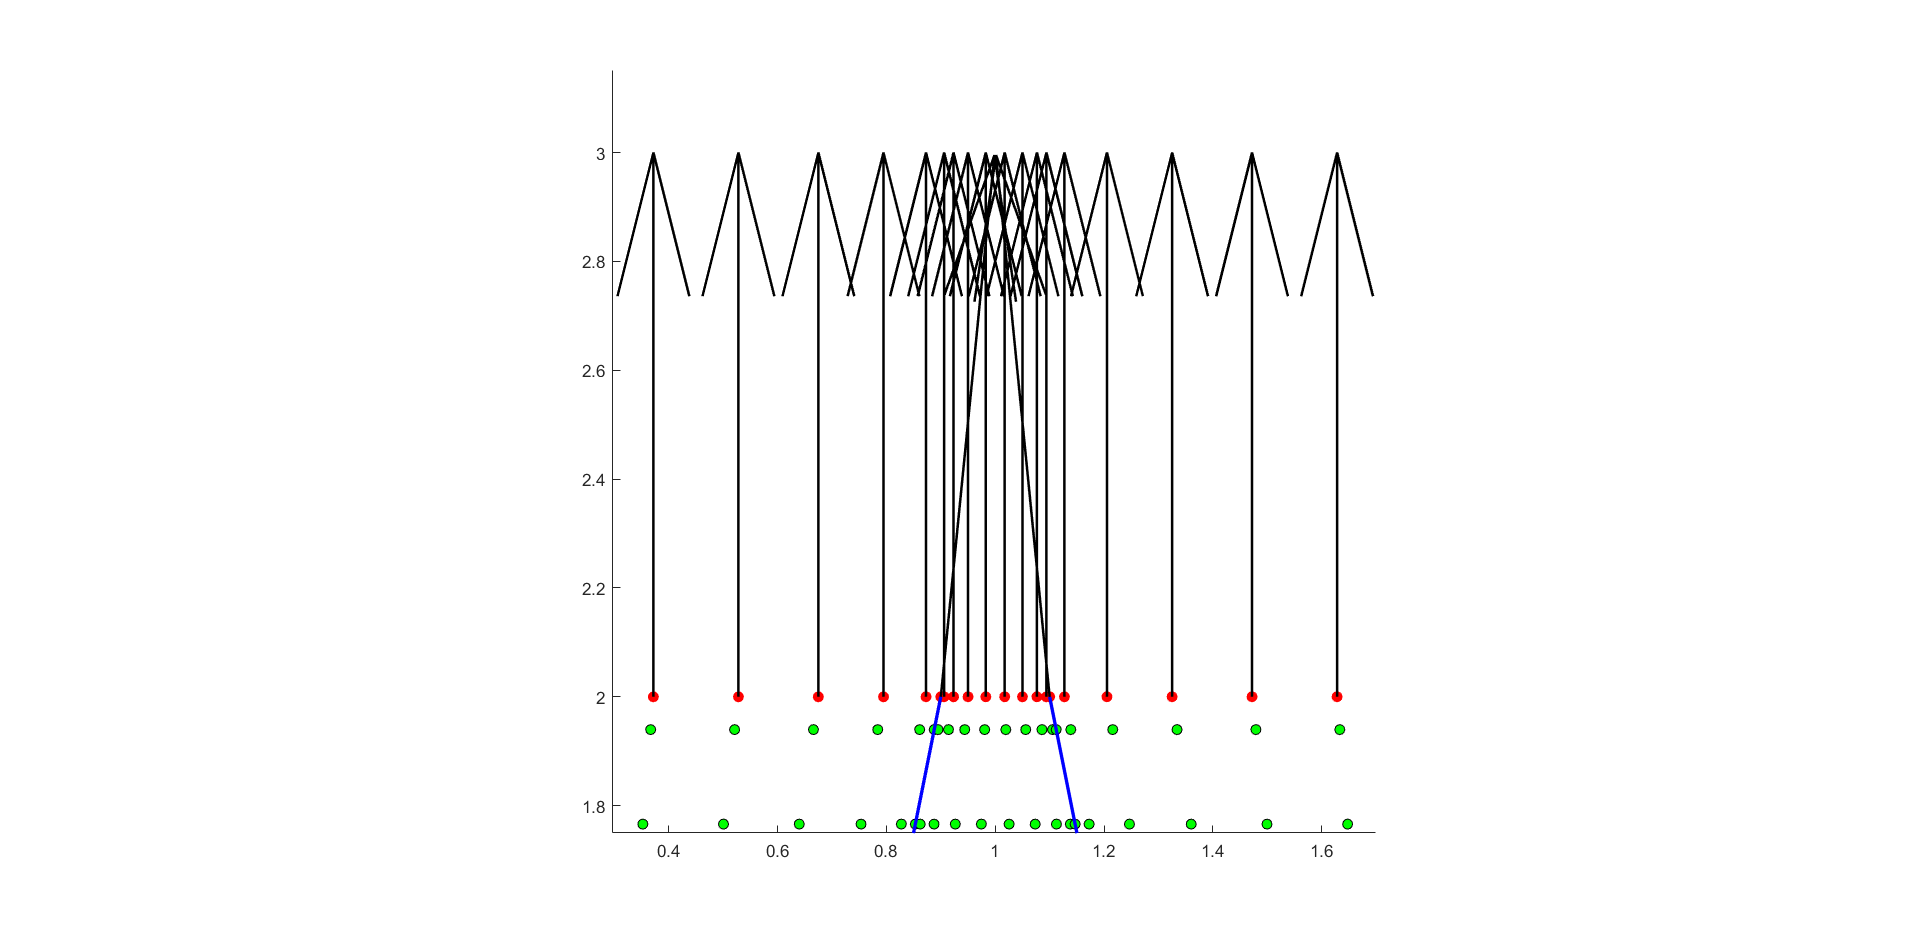
\includegraphics[scale=0.35]{F1.png}
%		\caption{Forward $\rho$ for $a = 0.01$} 
%		\label{F1}
%	\end{figure}

\begin{document}
	
	\begin{table}
		\centering
		\begin{tabular}{ | c | c | c | c | c | c | c ||}
			\hline
			& A.E. $ N=10$ & R.E. $N=10$ & A.E. $N = 20$ & R.E. $N = 20$ & A.E. $N=30$  & R.E. $N=30$ \\
			\hline
			\hline
			b & $\numprint{2.3315e-15}$ & $\numprint{2.5767e-15}$ & $\numprint{2.3315e-15}$ & $\numprint{2.5767e-15}$ & $\numprint{3.2196e-15}$ & $\numprint{3.5583e-15}$ \\
			f & $\numprint{2.2204e-15}$ & $\numprint{2.4540e-15}$ & $\numprint{2.7756e-15}$ & $\numprint{3.0675e-15}$ & $\numprint{3.2196e-15}$ & $\numprint{3.5583e-15}$ \\
			g & $\numprint{2.6645e-15}$ & $\numprint{2.9448e-15}$ & $\numprint{2.9976e-15}$ & $\numprint{3.3129e-15}$ & $\numprint{3.6637e-15}$ & $\numprint{4.0491e-15}$ \\
			j & $\numprint{1.6131e+00}$ & $\numprint{9.9560e-1}$ & $\numprint{1.6185e+00}$ & $\numprint{9.9890e-1}$ & $\numprint{1.5973e+00}$ & $\numprint{9.8583e-1}$ \\
			k & $\numprint{1.6186e+00}$ & $\numprint{9.9898e-1}$ & $\numprint{5.2237e-5}$ & $\numprint{3.2240e-5}$ & $\numprint{1.5018e+00}$ & $\numprint{9.2687e-1}$ \\
			\hline
		\end{tabular}
		\caption{Table Interp}
		\label{Tab:Interp}
	\end{table}
	
	
	
	\begin{figure}[h]
		\centering
		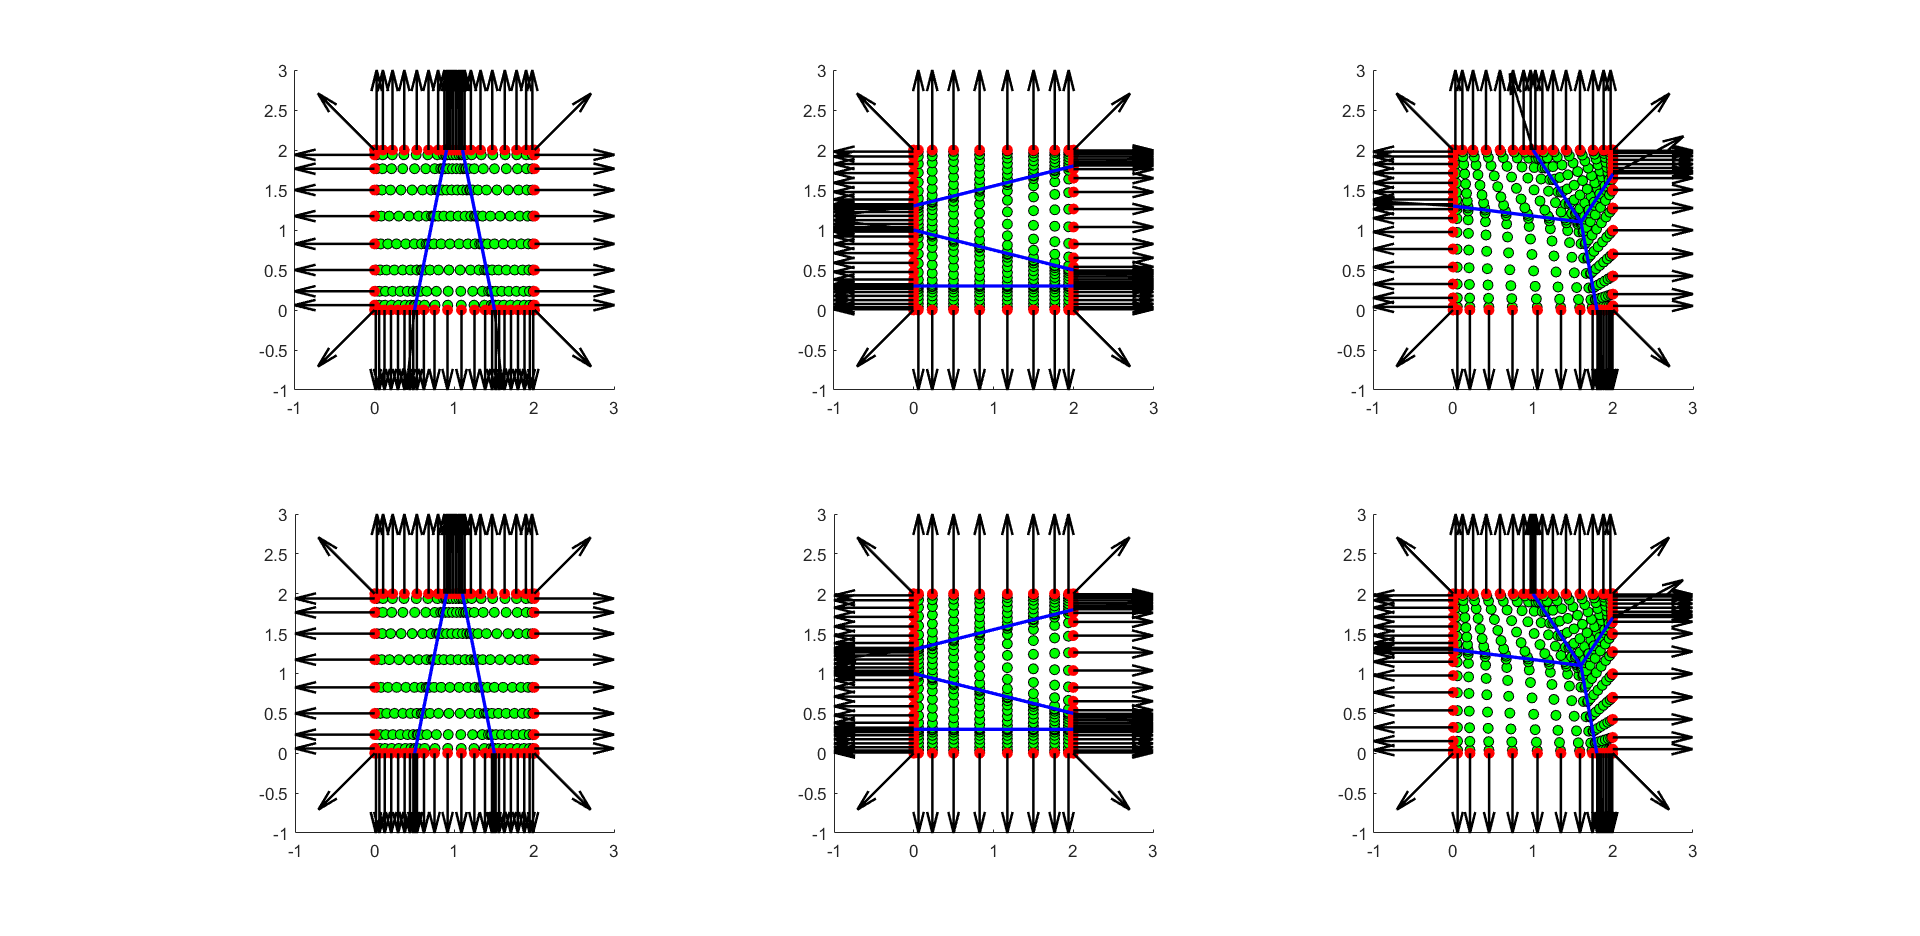
\includegraphics[scale=0.4]{NormalsNotFixed.png}
		\caption{Normal override (bottom) vs original normals (top)} 
		\label{F1}
	\end{figure}
\begin{figure}[h]
	\centering
	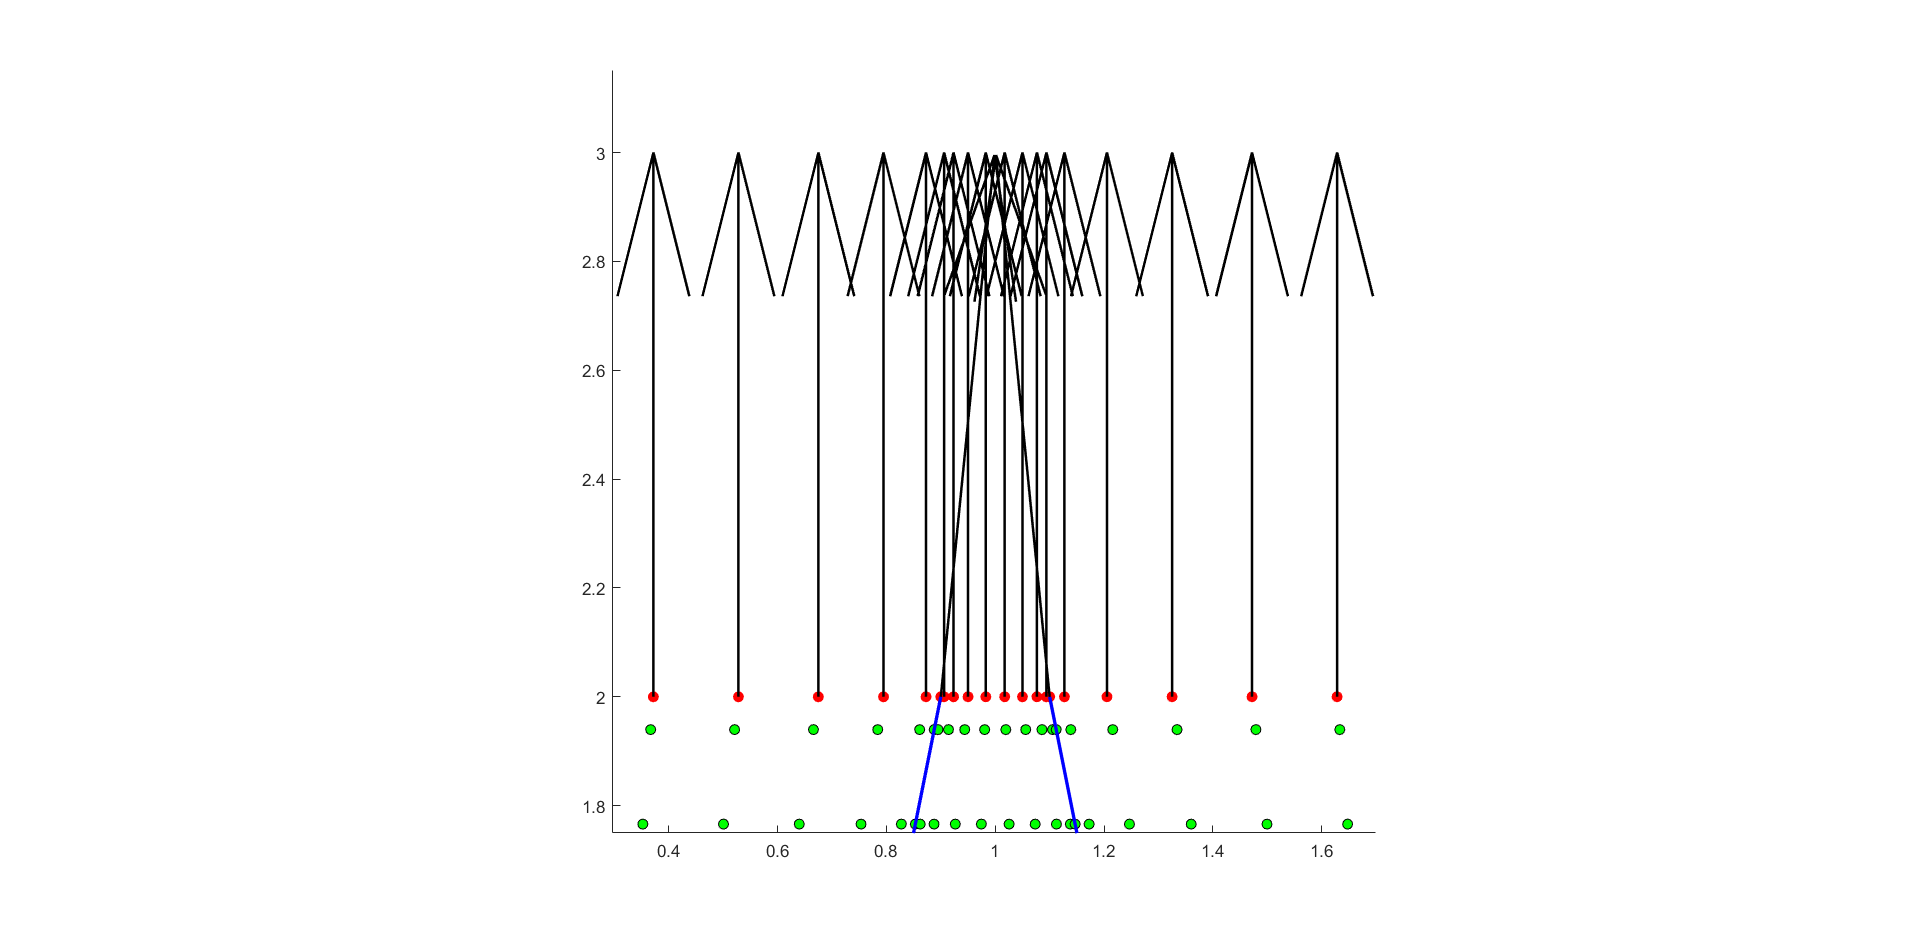
\includegraphics[scale=0.4]{F1.png}
	\caption{Discretization 1} 
	\label{F1a}
\end{figure}
\begin{figure}[h]
	\centering
	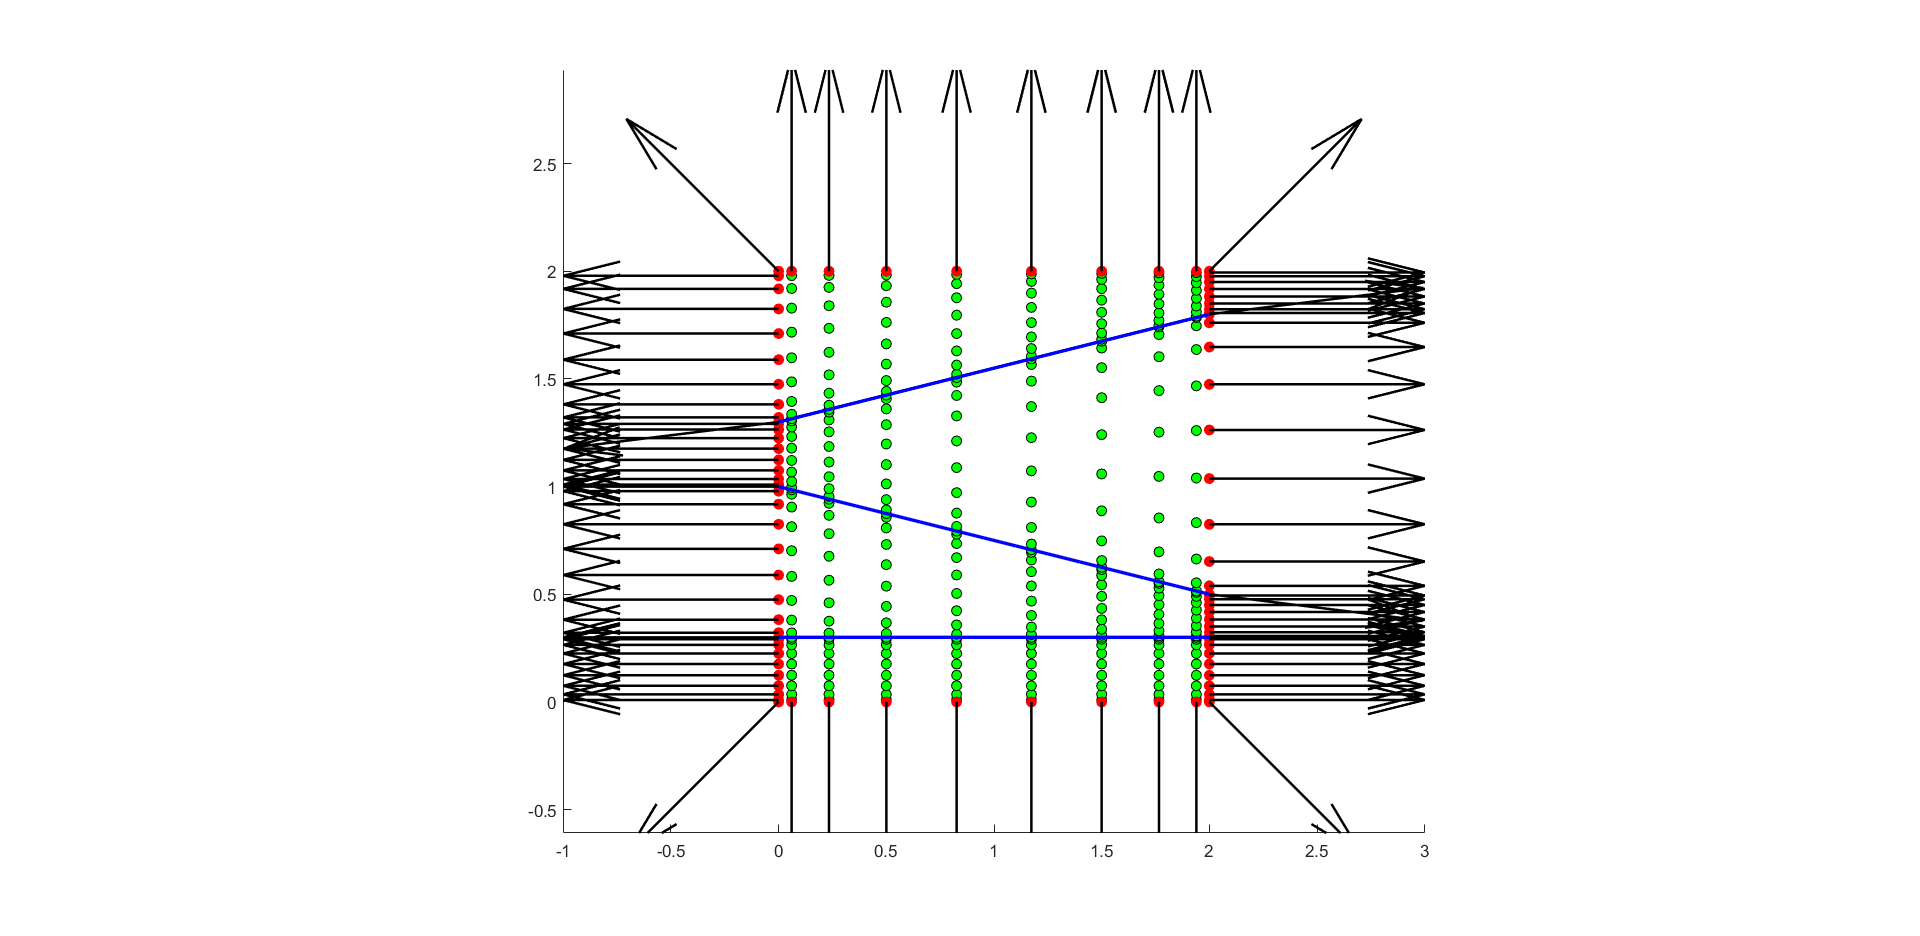
\includegraphics[scale=0.4]{F2.png}
	\caption{Discretization 2} 
	\label{F1b}
\end{figure}
\begin{figure}[h]
	\centering
	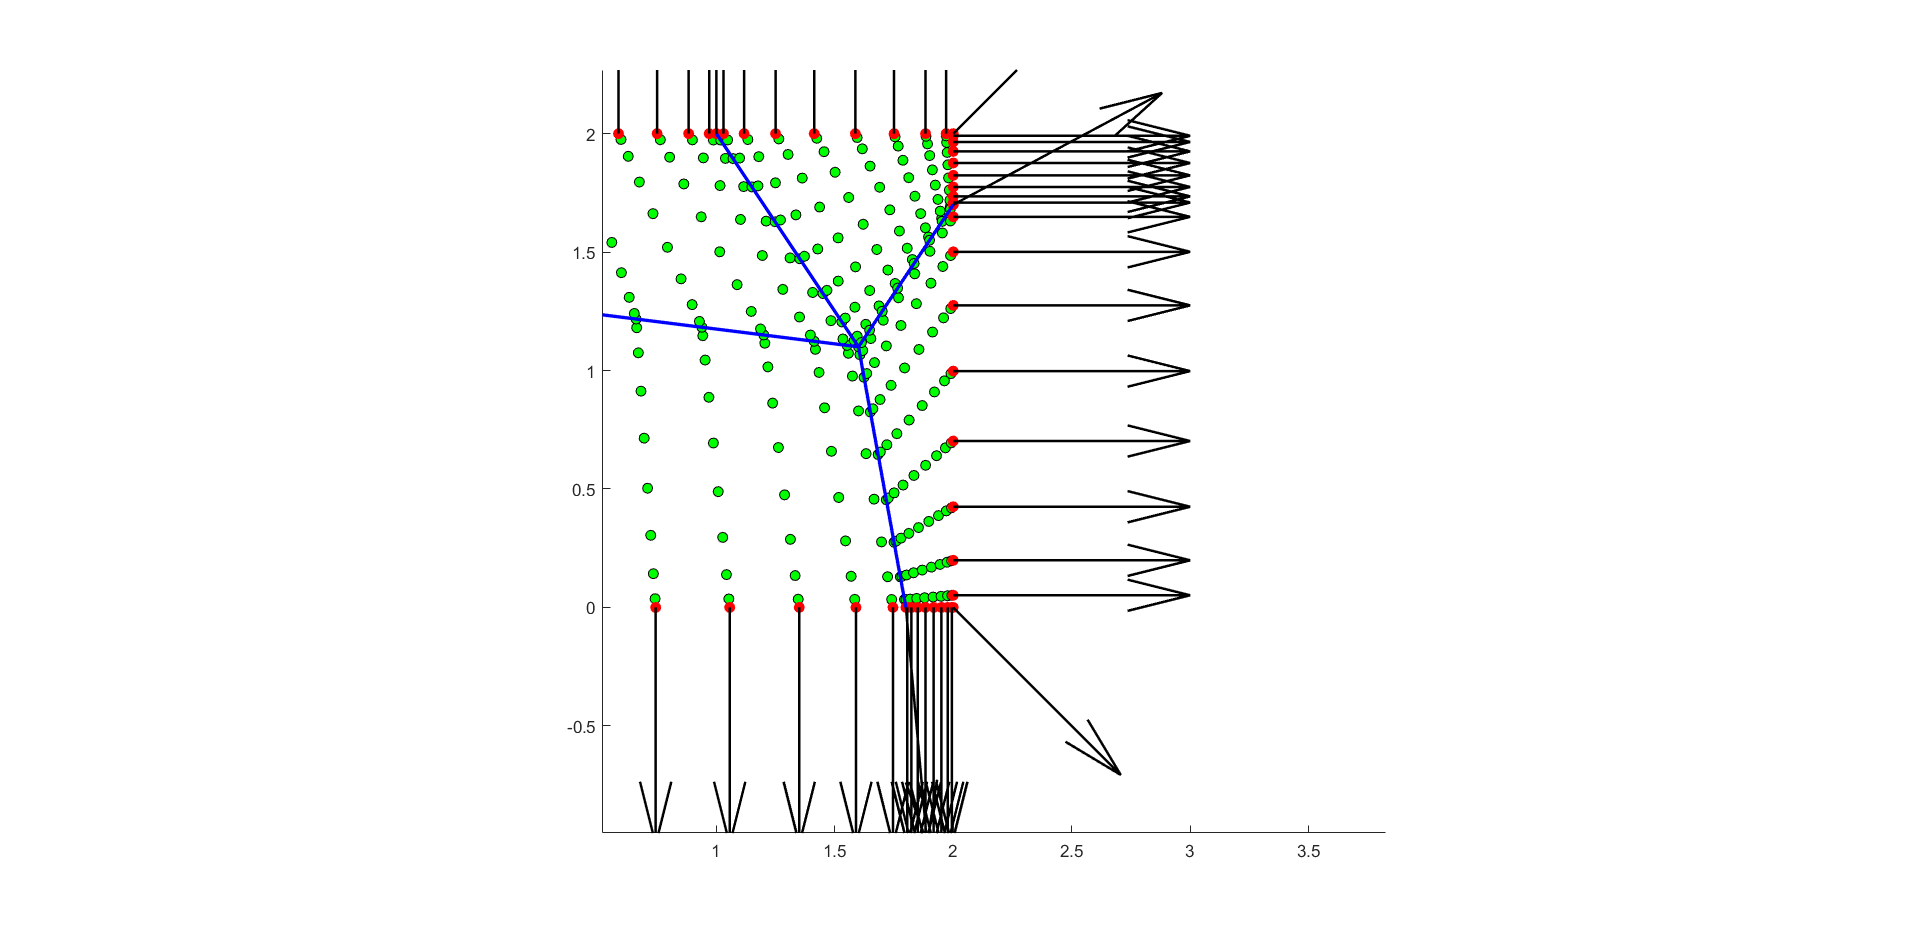
\includegraphics[scale=0.4]{F3.png}
	\caption{Discretization 3} 
	\label{F1c}
\end{figure}


Questions Mutishape:\\
\begin{itemize}
	\item Normal Overwriting, Figure \ref{F1} and 'zoom in' Figures \ref{F1a}, \ref{F1b} and \ref{F1c}.
	\item Interpolation testing (see below)
	\item InterpolationPhys Code, mapping to polars for all y
	\item Why is interpolation always in comp space
	\item Convolution in Multishape: Int for polars
	\item Why 2 matching conditions?
	\item FFT Interpolation formula
	\item Polar Diff at $r=0$?
	\item Wedge linear, quadrilateral bilinear. why?
	\item Algorithm writing...
\end{itemize}



If we interpolate from a multishape (b) onto itself we get an error of $0.1028$, however, if we plot the error it does not match, see Figure \ref{F2}. \\
When we interpolate both multishapes (a), (b) onto a uniform grid and plot the error, we get the error $ 0.1301$, which is displayed in Figure \ref{F3}.

\begin{figure}[h]
	\centering
	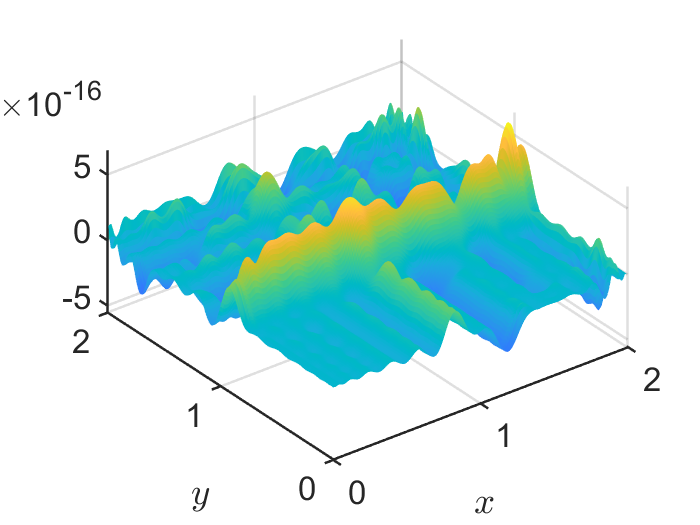
\includegraphics[scale=0.4]{ErrPhys.png}
	\caption{Error InterpPhys} 
	\label{F2}
\end{figure}

\begin{figure}[h]
	\centering
	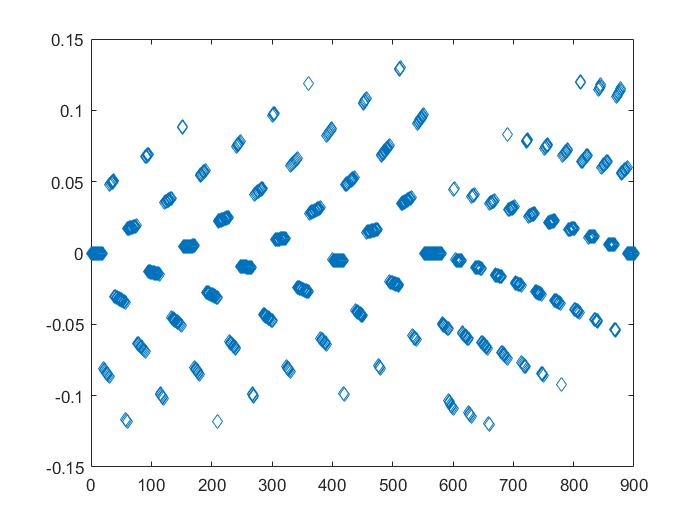
\includegraphics[scale=0.4]{ErrUni1.png}
	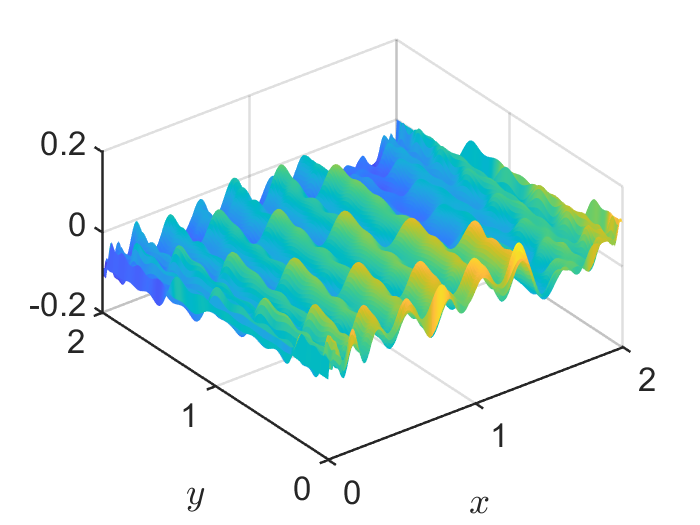
\includegraphics[scale=0.4]{ErrUni2.png}
	\caption{Error InterpUni} 
	\label{F3}
\end{figure}

\begin{table}
\centering
\begin{tabular}{ | c | c || c | c | c | c | c ||}
\hline
 & A.E. $ N=10$ & R.E. $N=10$ & A.E. $N = 20$ & R.E. $N = 20$ & A.E. $N=30$  & R.E. $N=30$ \\
\hline
\hline
 b & $\numprint{0.0000e+00}$ & $\numprint{0.0000e+00}$ & $\numprint{4.4409e-16}$ & $\numprint{1.4937e-16}$ & $\numprint{8.8818e-16}$ & $\numprint{2.9873e-16}$ \\
 f & $\numprint{0.0000e+00}$ & $\numprint{0.0000e+00}$ & $\numprint{0.0000e+00}$ & $\numprint{0.0000e+00}$ & $\numprint{8.8818e-16}$ & $\numprint{2.9873e-16}$ \\
 g & $\numprint{0.0000e+00}$ & $\numprint{0.0000e+00}$ & $\numprint{4.4409e-16}$ & $\numprint{1.4937e-16}$ & $\numprint{8.8818e-16}$ & $\numprint{2.9873e-16}$ \\
 j & $\numprint{2.4085e-8}$ & $\numprint{3.7621e-9}$ & $\numprint{1.7764e-15}$ & $\numprint{2.7746e-16}$ & $\numprint{2.6645e-15}$ & $\numprint{4.1620e-16}$ \\
 k & $\numprint{2.7334e-11}$ & $\numprint{4.2695e-12}$ & $\numprint{1.7764e-15}$ & $\numprint{2.7746e-16}$ & $\numprint{1.7764e-15}$ & $\numprint{2.7746e-16}$ \\
\hline
\end{tabular}
\caption{Table Int}
\label{Tab:Int}
\end{table}


Not related to multishape: Is DDFT valid for $\w$ which is not $\nabla V$?\\
DDFT Talk: What to focus on?


\end{document}